\documentclass[10pt,a4paper]{article}
\usepackage[T2A]{fontenc}    
\usepackage[english]{babel}   
\usepackage{color}
\usepackage[urlbordercolor={1 1 1},colorlinks=true]{hyperref}
\usepackage{longtable}
\usepackage{graphicx}
\usepackage[a4paper,left=2.5cm,right=2cm,top=2cm,bottom=2cm]{geometry}

\usepackage{mathptmx}
\usepackage{arev}
\usepackage{indentfirst}
% \usepackage[default,osfigures,scale=0.95]{opensans}
% \usepackage[defaultsans]{droidsans}
% \usepackage{fontspec}
% \renewcommand{\sfdefault}{phv}
% \renewcommand{\sfdefault}{PTSansCaption-TLF}
% \fontfamily{pag}\selectfont
% \renewcommand{\rmdefault}{\sfdefault}
% \renewcommand{\rmdefault}{ptm}
% \setmainfont{Times}
% \fontfamily{Name_OF_Font_Family}\selectfont


%\input{newcommands}
\definecolor{link}{rgb}{0,0,0.6}

\hypersetup
{
	linkcolor=link,
	urlcolor={link}
}

\newcommand{\lmpratio}{0.15}
\newcommand{\rmpratio}{0.74}
\newcommand{\verticalSpace}{0.3cm}
\newcommand{\vSpace}{0.5cm}
\newcommand{\horizontalSpace}{0.05\textwidth}

\newcommand{\sectionTitle}[1]{\Large{\textbf{#1}}}
\newcommand{\sectionMain}[1]{\textbf{#1}}

\newcommand{\vacancyName}{PhD student}
\renewcommand*\familydefault{\sfdefault}
% \renewcommand{\familydefault}{\sfdefault}


\setlength{\parindent}{3em}
\setlength{\parskip}{0.5em}

\begin{document}

	\pagenumbering{gobble} 
	

	\raggedright{\Large{\textbf{Arseniy Shchepetnov}}}\\[0.3cm]
	
	\begin{minipage}[t]{0.7\textwidth}
		\vspace{0pt}
		\raggedright{\textbf{Lead Data Scientist}}\\[0.3cm]
		% 	\raggedright{\huge\vacancyName}\\[0.3cm]
		% 	\noindent Date of birth: $15^{\mathrm{th}}$ December $1989$ \\[0.1cm]
		\noindent Address: Saint-Petersburg, Russian Federation \\[0.1cm]
		\noindent Email: \href{mailto:a.shchepetnov@gmail.com}{a.shchepetnov@gmail.com}\\[0.1cm]
		\noindent Phone: $+7\,953\,149\,42\,68$ \\
		\noindent GitHub: \href{https://github.com/ArseniyShchepetnov}{ArseniyShchepetnov}\\
            \noindent LinkedIn: \href{https://www.linkedin.com/in/arseniy-shchepetnov-4a236171/}{Arseniy Shchepetnov}\\
            \noindent Medium: \href{https://medium.com/@a.shchepetnov}{Arseniy Shchepetnov}
	\end{minipage}
	\begin{minipage}[t]{0.2\textwidth}
		\vspace{0pt}
		% 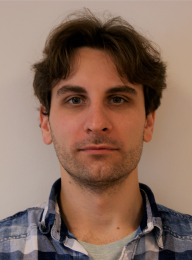
\includegraphics[width=\linewidth]{photo.png}
	\end{minipage}
	
	
	\section*{Objective}
	
	Data Science/Lead Data Science, Development
	
	\section*{Relevant skills}
	
	\setlength{\parindent}{3em}

	
My interest vector is referred to Data Science, Research and Development, Product Development related to technologies.
5 years of academic research in Theoretical Physics (quantum physics) provided a fundamental pillar and a useful tool for my development in Data Science.
I have more than 8 years of development practice with different languages learning to write structured and maintanable code.
For a long time I have been working in agile format and participated in product development. 


I have advanced development skills with Python including linting and CI/CD (see examples on GitHub).
Other languages that are covered with my experience are C++, Fortran, R.
In different organizations I gained experience in Digital Signal Processing, Machine Learning, Deep Learning, etc, and I have developed many product components and algorithmic solutions for business value, that were successfully deployed. 
Under my direction a new data processing service was developed for the analysis of geological data using deep learning models.
For the last few years, I've been working as a Team Leader Data Scientist at multiple projects.

	

	
	\setlength{\parindent}{0em}
	\vspace{\verticalSpace}
%-------------------------------------------------------------------------------------------------------------------------------	
	\vspace{\verticalSpace}
	\section*{Employment history}



	% PWC
	\begin{minipage}[t]{\lmpratio\textwidth}
		May 2021 --- \\Now
	\end{minipage}
	\hspace{\horizontalSpace}
	\begin{minipage}[t]{\rmpratio\textwidth}
		\sectionMain{Lead Data Scientist/Team Lead/Senior Consultant}\\
		\href{https://www.pwc.ru/}{<<PWC>>} (Technology, Artificial Intelligence), Saint-Petersburg\\[0.1cm]		
		
		\begin{itemize}
                \item 
I am leading two projects based on bayesian networks and deep learning models and two teams at the projects.
			\item 
For template-based bayesian networks I developed microservice for the product, designed numerical methods optimizations and metodology extensions.
All solutions are deployed to the product at the client.   
			\item 
For well logs data analysis I designed infrastructure and the client service with deep learning models.
Under my direction the team solved multiple tasks related to oil intervals detection, GIS retrieval and spatial analysis.
			\item 
Also, I take part in team and product development, buisness development, hiring process, contacting with other organizations and universities etc.

		\end{itemize}
		
		After rebranding in July the unit is called <<Digital Formula of Trust>> and I was promoted up to the manager grade.
		
	\end{minipage}	
	\vspace{\vSpace}
	
	% IBM
	\begin{minipage}[t]{\lmpratio\textwidth}
		May 2018 --- \\May 2021
	\end{minipage}
	\hspace{\horizontalSpace}
	\begin{minipage}[t]{\rmpratio\textwidth}
		\sectionMain{Data Scientist/Lead Data Scientist/Team Lead}\\
		\href{https://www.ibm.com/ru/rstl/index-en.html}{<<IBM STC>>} (GBS, ``Cognitive Practice Team''), Saint-Petersburg, Moscow\\[0.5cm]		
		
  
		\begin{itemize}
                \item 
I was working on data engeneering solutions including geological data processing and ML solutions development in a team.
We developed models which found productive intervals which resulted in oil extraction.
                \item 
I carried out research in correlation of wells for spatial analysis and designed several models.
With developed models correlation prediction were made for the client.
                \item
I developed multiple model and data serving solutions for deep learning models in geology.
                

            \end{itemize}
		
	\end{minipage}	
	\vspace{\vSpace}
	
	% Healbe
	\begin{minipage}[t]{\lmpratio\textwidth}
		Aug 2016 --- \\May 2018
	\end{minipage}
	\hspace{\horizontalSpace}
	\begin{minipage}[t]{\rmpratio\textwidth}
		\sectionMain{Research and Development}\\
		\href{https://healbe.com/}{<<Healbe corp.>>}, Saint-Petersburg\\[0.5cm]		
		\begin{itemize}
                \item 
I developed algorithms for costom piezoelectric and optical devices which were successfully deployed.
                \item 
I developed several utilities for data transfer from warable devices and applying algorithms on the local machine which were used also in parallel projects.
            \end{itemize}
		 
		
	\end{minipage}	
	\vspace{\vSpace}
	
	% SPBSU	
	\begin{minipage}[t]{\lmpratio\textwidth}
		Jan 2015 --- \\Dec 2015
	\end{minipage}
	\hspace{\horizontalSpace}
	\begin{minipage}[t]{\rmpratio\textwidth}
		\sectionMain{Researcher}\\
		\href{http://english.spbu.ru/}{<<Saint-Petersburg State University>>}, Saint-Petersburg\\[0.5cm]		
		Research in the field of atomic physics. 
		Main themes: $g$ factor theory, nuclear recoil effect. \\

	\end{minipage}
	\vspace{\vSpace}

	\begin{minipage}[t]{\lmpratio\textwidth}
		Jan 2014 --- \\Dec 2016
	\end{minipage}
	\hspace{\horizontalSpace}
	\begin{minipage}[t]{\rmpratio\textwidth}
		\sectionMain{Researcher}\\
		\href{http://frrc.itep.ru/index.php/en/}{<<Institute for Theoretical and Experimental Physics>>}, Moscow\\[0.5cm]
		Research in the field of atomic physics supported by ``Helmholtz-Rosatom'' grant. 
		Theme: ``Zeeman splitting in highly-charged ions: novel approach to the non-linear effects''. \\[0.5cm]
		
	\end{minipage}
	
	\vspace{\vSpace}

	\begin{minipage}[t]{\lmpratio\textwidth}
		Nov 2013 --- \\Feb 2016
	\end{minipage}
	\hspace{\horizontalSpace}
	\begin{minipage}[t]{\rmpratio\textwidth}
		\sectionMain{Engineer-programmer}\\
		\href{http://www.rimr.ru/eng/}{<<Russian Institute for Power Radiobuilding>>}, Saint-Petersburg\\[0.5cm]
            \begin{itemize}
                \item
I developed PostgreSQL database and UI on C++/Qt4 which was successfully deployed for buisness on Linux.
            \end{itemize}

	\end{minipage}

		\vspace{\vSpace}
	
	\begin{minipage}[t]{\lmpratio\textwidth}
		Sep 2011 --- \\Jan 2012
	\end{minipage}
	\hspace{\horizontalSpace}
	\begin{minipage}[t]{\rmpratio\textwidth}
		\sectionMain{Teacher (Physics)}\\
		\href{http://lnmo.ru/}{<<Laboratory for Continuous Mathematical Education>>}, Saint-Petersburg\\[0.5cm]
		Teaching physics at 8 and 9 year classes. Special seminars on thermodynamics.
	\end{minipage}	
	\vspace{\verticalSpace}
%-------------------------------------------------------------------------------------------------------------------------------
	\vspace{\verticalSpace}
	\section*{Education}
	
	\begin{minipage}[t]{\lmpratio\textwidth}
		Sep 2013 --- \\Jul 2016
	\end{minipage}
	\hspace{\horizontalSpace}
	\begin{minipage}[t]{\rmpratio\textwidth}
		\sectionMain{Postgraduate student} (Theoretical Physics)\\[0.1cm]		
		\href{http://english.spbu.ru/}{Saint-Petersburg State University}\\ Department of Physics, Division of Quantum Mechanics\\[0.3cm]
		 Thesis: ``Nuclear recoil corrections to the $g$ factor of highly-charged ions'' \\[0.3cm]
		 Scientific advisors: \href{http://fock.phys.spbu.ru/english/tupicin_en.htm}{Prof. Ilya Tupitsyn} and \href{http://fock.phys.spbu.ru/glazov.htm}{Dr. Dmitry Glazov}
	\end{minipage}

	\vspace{1cm}
	
	\begin{minipage}[t]{\lmpratio\textwidth}
		Sep 2011 --- \\Jul 2013
	\end{minipage}
	\hspace{\horizontalSpace}
	\begin{minipage}[t]{\rmpratio\textwidth}
		\sectionMain{Master's degree} (Quantum Mechanics of Atoms, Molecules and Solids) \\[0.1cm]
		\href{http://english.spbu.ru/}{Saint-Petersburg State University}\\ Department of Physics, Division of Quantum Mechanics\\[0.3cm]
		 Thesis: ``Nuclear recoil corrections to the energy levels and to the $g$ factor of highly-charged ions''\\[0.3cm]
		 Scientific advisor: \href{http://fock.phys.spbu.ru/english/tupicin_en.htm}{Prof. Ilya Tupitsyn} and \href{http://fock.phys.spbu.ru/glazov.htm}{Dr. Dmitry Glazov}
	\end{minipage}

	\vspace{1cm}
	
	\begin{minipage}[t]{\lmpratio\textwidth}
		Sep 2007 --- \\Jul 2011
	\end{minipage}
	\hspace{\horizontalSpace}
	\begin{minipage}[t]{\rmpratio\textwidth}
		\sectionMain{Bachelor's degree} (Quantum Mechanics of Atoms, Molecules and Solids) \\[0.1cm]
		\href{http://english.spbu.ru/}{Saint-Petersburg State University}\\ Department of Physics, Division of Quantum Mechanics\\[0.3cm]
		 Thesis: ``Nuclear recoil corrections to the energy levels of highly-charged ions''\\[0.3cm]
		 Scientific advisor: \href{http://fock.phys.spbu.ru/english/shabaev_en.htm}{Prof. Vladimir Shabaev}
	\end{minipage}
	
	\newpage
	
%-------------------------------------------------------------------------------------------------------------------------------
	\section*{Certificates}	

        \begin{minipage}[t]{\lmpratio\textwidth}
		Coursera\\August 2022
	\end{minipage}
	\hspace{\horizontalSpace}
	\begin{minipage}[t]{\rmpratio\textwidth}
		\sectionMain{Natural Language Processing Specialization}\\
            \href{https://www.coursera.org/account/accomplishments/specialization/certificate/D4F2WRLEHCY8}{D4F2WRLEHCY8}
	\end{minipage}
	\vspace{1cm}

        \begin{minipage}[t]{\lmpratio\textwidth}
		Coursera\\August 2022
	\end{minipage}
	\hspace{\horizontalSpace}
	\begin{minipage}[t]{\rmpratio\textwidth}
		\sectionMain{Natural Language Processing with Attention Models}\\
		\href{https://www.coursera.org/account/accomplishments/certificate/TT5J2NHDYDY2}{TT5J2NHDYDY2}
	\end{minipage}
	\vspace{1cm}

	\begin{minipage}[t]{\lmpratio\textwidth}
		Coursera\\August 2022
	\end{minipage}
	\hspace{\horizontalSpace}
	\begin{minipage}[t]{\rmpratio\textwidth}
		\sectionMain{Natural Language Processing with Classification and Vector Spaces}\\
		\href{https://www.coursera.org/account/accomplishments/certificate/3LL65SQH6EWM}{3LL65SQH6EWM}
	\end{minipage}
	\vspace{1cm}

	\begin{minipage}[t]{\lmpratio\textwidth}
		Coursera\\August 2022
	\end{minipage}
	\hspace{\horizontalSpace}
	\begin{minipage}[t]{\rmpratio\textwidth}
		\sectionMain{Natural Language Processing with Probabilistic Models}\\
		\href{https://www.coursera.org/account/accomplishments/certificate/C3RSRG7T853E}{C3RSRG7T853E}
	\end{minipage}
	\vspace{1cm}
	

	\begin{minipage}[t]{\lmpratio\textwidth}
		Coursera\\August 2022
	\end{minipage}
	\hspace{\horizontalSpace}
	\begin{minipage}[t]{\rmpratio\textwidth}
		\sectionMain{Natural Language Processing with Sequence Models}\\
		\href{https://www.coursera.org/account/accomplishments/certificate/667D47FVSK3M}{667D47FVSK3M}
	\end{minipage}
	\vspace{1cm}


	\begin{minipage}[t]{\lmpratio\textwidth}
		Coursera\\July 2022
	\end{minipage}
	\hspace{\horizontalSpace}
	\begin{minipage}[t]{\rmpratio\textwidth}
		\sectionMain{Combinatorics and Probability}\\
		\href{https://www.coursera.org/account/accomplishments/certificate/EFYQQQ9GUTUP}{EFYQQQ9GUTUP}
	\end{minipage}
	\vspace{1cm}

	\begin{minipage}[t]{\lmpratio\textwidth}
		Coursera\\June 2022
	\end{minipage}
	\hspace{\horizontalSpace}
	\begin{minipage}[t]{\rmpratio\textwidth}
		\sectionMain{Sample-based Learning Methods}\\
		\href{https://www.coursera.org/account/accomplishments/certificate/KC4T942AATVE}{KC4T942AATVE}
	\end{minipage}
	\vspace{1cm}

		
	\begin{minipage}[t]{\lmpratio\textwidth}
		Coursera\\May 2022
	\end{minipage}
	\hspace{\horizontalSpace}
	\begin{minipage}[t]{\rmpratio\textwidth}
		\sectionMain{Fundamentals of Reinforcement Learning}\\
		\href{https://www.coursera.org/account/accomplishments/certificate/U3NT5V7XZCNK}{U3NT5V7XZCNK}
	\end{minipage}
	\vspace{1cm}
		
	
%-------------------------------------------------------------------------------------------------------------------------------
	\section*{Publications}
	\begin{itemize}
		\item A.~A.~Shchepetnov, D.~A.~Glazov, A.~V.~Volotka, V.~M.~Shabaev, I.~I.~Tupitsyn, G.~Plunien 
			``Nuclear recoil correction to the $g$ factor of boron-like argon''. Journal of Physics: Conference Series, 2015. --- Vol. 583, --- P. 012001
		\item I.~A.~Aleksandrov, A.~A.~Shchepetnov, D.~A.~Glazov, V.~M.~Shabaev 
			``Finite nuclear size corrections to the recoil effect in hydrogenlike ions''. Journal of Physics B: Atomic, Molecular and Optical Physics, 2015. --- Vol. 48, --- No. 14. --- P. 144004		
		\item D.~A.~Glazov, A.~V.~Volotka, A.~A.~Schepetnov, M.~M.~Sokolov, V.~M.~Shabaev, I.~I.~Tupitsyn, G.~Plunien 
			``$g$ factor of boron-like ions: ground and excited states''. Physica Scripta, 2013. --- Vol. T156, --- P. 014014
	\end{itemize}
% 	New articles are in preparation. 
% 	\vspace{\verticalSpace}
% 	\newpage
	\section*{International conferences}
		\begin{itemize}
			\item[---]	Seminar on Astrophysics, Clocks and Fundamental Constants, Bad Honnef, Germany (Poster), 2015
			\item[---]	Topical Workshop of the SPARC Collaboration, Worms, Germany (Poster), 2014
			\item[---]	\href{http://indico.gsi.de/conferenceDisplay.py?confId=2443}{International Conference on Science and Technology for FAIR}, Worms, Germany (Poster), 2014
			\item[---]	\href{http://www.cab.cnea.gov.ar/hci2014/}{International Conference on the Physics of Highly Charged Ions}, San Carlos de Bariloche, Argentina (\textbf{Oral presentation}), 2014
			\item[---]	\href{https://sites.google.com/site/finqinternational/home}{Fin Q workshop}: International conference <<Quantum Informatics and Applications>>, St. Petersburg, Russia (No report), 2013
			\item[---]	\href{http://www.gao.spb.ru/russian/psas/ffk2013/}{The Workshop on Precision Physics and Fundamental Physical Constants}, Pulkovo, St. Petersburg, Russia (Poster), 2013
			\item[---]	\href{http://fas.vsu.ru/en/index.php}{XX Conference on Fundamental Atomic Spectroscopy}, Voronezh, Russia (\textbf{Oral presentation}), 2013
		\end{itemize}		
	
	\vspace{5cm}
	
	Arseniy Shchepetnov
	
	
	
	
\end{document}

